% Options for packages loaded elsewhere
\PassOptionsToPackage{unicode}{hyperref}
\PassOptionsToPackage{hyphens}{url}
\PassOptionsToPackage{dvipsnames,svgnames*,x11names*}{xcolor}
%
\documentclass[
]{article}
\usepackage{lmodern}
\usepackage{amssymb,amsmath}
\usepackage{ifxetex,ifluatex}
\ifnum 0\ifxetex 1\fi\ifluatex 1\fi=0 % if pdftex
  \usepackage[T1]{fontenc}
  \usepackage[utf8]{inputenc}
  \usepackage{textcomp} % provide euro and other symbols
\else % if luatex or xetex
  \usepackage{unicode-math}
  \defaultfontfeatures{Scale=MatchLowercase}
  \defaultfontfeatures[\rmfamily]{Ligatures=TeX,Scale=1}
\fi
% Use upquote if available, for straight quotes in verbatim environments
\IfFileExists{upquote.sty}{\usepackage{upquote}}{}
\IfFileExists{microtype.sty}{% use microtype if available
  \usepackage[]{microtype}
  \UseMicrotypeSet[protrusion]{basicmath} % disable protrusion for tt fonts
}{}
\makeatletter
\@ifundefined{KOMAClassName}{% if non-KOMA class
  \IfFileExists{parskip.sty}{%
    \usepackage{parskip}
  }{% else
    \setlength{\parindent}{0pt}
    \setlength{\parskip}{6pt plus 2pt minus 1pt}}
}{% if KOMA class
  \KOMAoptions{parskip=half}}
\makeatother
\usepackage{xcolor}
\IfFileExists{xurl.sty}{\usepackage{xurl}}{} % add URL line breaks if available
\IfFileExists{bookmark.sty}{\usepackage{bookmark}}{\usepackage{hyperref}}
\hypersetup{
  pdftitle={Box Office Blues},
  pdfauthor={STAT-420, Team: Summer Proj, A Arora, S Dani, G Shrivastava},
  colorlinks=true,
  linkcolor=Maroon,
  filecolor=Maroon,
  citecolor=Blue,
  urlcolor=cyan,
  pdfcreator={LaTeX via pandoc}}
\urlstyle{same} % disable monospaced font for URLs
\usepackage[margin=1in]{geometry}
\usepackage{color}
\usepackage{fancyvrb}
\newcommand{\VerbBar}{|}
\newcommand{\VERB}{\Verb[commandchars=\\\{\}]}
\DefineVerbatimEnvironment{Highlighting}{Verbatim}{commandchars=\\\{\}}
% Add ',fontsize=\small' for more characters per line
\usepackage{framed}
\definecolor{shadecolor}{RGB}{248,248,248}
\newenvironment{Shaded}{\begin{snugshade}}{\end{snugshade}}
\newcommand{\AlertTok}[1]{\textcolor[rgb]{0.94,0.16,0.16}{#1}}
\newcommand{\AnnotationTok}[1]{\textcolor[rgb]{0.56,0.35,0.01}{\textbf{\textit{#1}}}}
\newcommand{\AttributeTok}[1]{\textcolor[rgb]{0.77,0.63,0.00}{#1}}
\newcommand{\BaseNTok}[1]{\textcolor[rgb]{0.00,0.00,0.81}{#1}}
\newcommand{\BuiltInTok}[1]{#1}
\newcommand{\CharTok}[1]{\textcolor[rgb]{0.31,0.60,0.02}{#1}}
\newcommand{\CommentTok}[1]{\textcolor[rgb]{0.56,0.35,0.01}{\textit{#1}}}
\newcommand{\CommentVarTok}[1]{\textcolor[rgb]{0.56,0.35,0.01}{\textbf{\textit{#1}}}}
\newcommand{\ConstantTok}[1]{\textcolor[rgb]{0.00,0.00,0.00}{#1}}
\newcommand{\ControlFlowTok}[1]{\textcolor[rgb]{0.13,0.29,0.53}{\textbf{#1}}}
\newcommand{\DataTypeTok}[1]{\textcolor[rgb]{0.13,0.29,0.53}{#1}}
\newcommand{\DecValTok}[1]{\textcolor[rgb]{0.00,0.00,0.81}{#1}}
\newcommand{\DocumentationTok}[1]{\textcolor[rgb]{0.56,0.35,0.01}{\textbf{\textit{#1}}}}
\newcommand{\ErrorTok}[1]{\textcolor[rgb]{0.64,0.00,0.00}{\textbf{#1}}}
\newcommand{\ExtensionTok}[1]{#1}
\newcommand{\FloatTok}[1]{\textcolor[rgb]{0.00,0.00,0.81}{#1}}
\newcommand{\FunctionTok}[1]{\textcolor[rgb]{0.00,0.00,0.00}{#1}}
\newcommand{\ImportTok}[1]{#1}
\newcommand{\InformationTok}[1]{\textcolor[rgb]{0.56,0.35,0.01}{\textbf{\textit{#1}}}}
\newcommand{\KeywordTok}[1]{\textcolor[rgb]{0.13,0.29,0.53}{\textbf{#1}}}
\newcommand{\NormalTok}[1]{#1}
\newcommand{\OperatorTok}[1]{\textcolor[rgb]{0.81,0.36,0.00}{\textbf{#1}}}
\newcommand{\OtherTok}[1]{\textcolor[rgb]{0.56,0.35,0.01}{#1}}
\newcommand{\PreprocessorTok}[1]{\textcolor[rgb]{0.56,0.35,0.01}{\textit{#1}}}
\newcommand{\RegionMarkerTok}[1]{#1}
\newcommand{\SpecialCharTok}[1]{\textcolor[rgb]{0.00,0.00,0.00}{#1}}
\newcommand{\SpecialStringTok}[1]{\textcolor[rgb]{0.31,0.60,0.02}{#1}}
\newcommand{\StringTok}[1]{\textcolor[rgb]{0.31,0.60,0.02}{#1}}
\newcommand{\VariableTok}[1]{\textcolor[rgb]{0.00,0.00,0.00}{#1}}
\newcommand{\VerbatimStringTok}[1]{\textcolor[rgb]{0.31,0.60,0.02}{#1}}
\newcommand{\WarningTok}[1]{\textcolor[rgb]{0.56,0.35,0.01}{\textbf{\textit{#1}}}}
\usepackage{graphicx,grffile}
\makeatletter
\def\maxwidth{\ifdim\Gin@nat@width>\linewidth\linewidth\else\Gin@nat@width\fi}
\def\maxheight{\ifdim\Gin@nat@height>\textheight\textheight\else\Gin@nat@height\fi}
\makeatother
% Scale images if necessary, so that they will not overflow the page
% margins by default, and it is still possible to overwrite the defaults
% using explicit options in \includegraphics[width, height, ...]{}
\setkeys{Gin}{width=\maxwidth,height=\maxheight,keepaspectratio}
% Set default figure placement to htbp
\makeatletter
\def\fps@figure{htbp}
\makeatother
\setlength{\emergencystretch}{3em} % prevent overfull lines
\providecommand{\tightlist}{%
  \setlength{\itemsep}{0pt}\setlength{\parskip}{0pt}}
\setcounter{secnumdepth}{-\maxdimen} % remove section numbering
\usepackage{booktabs}
\usepackage{longtable}
\usepackage{array}
\usepackage{multirow}
\usepackage{wrapfig}
\usepackage{float}
\usepackage{colortbl}
\usepackage{pdflscape}
\usepackage{tabu}
\usepackage{threeparttable}
\usepackage{threeparttablex}
\usepackage[normalem]{ulem}
\usepackage{makecell}
\usepackage{xcolor}

\title{Box Office Blues}
\author{STAT-420, Team: Summer Proj, A Arora, S Dani, G Shrivastava}
\date{July 2020}

\begin{document}
\maketitle

\begin{center}\rule{0.5\linewidth}{0.5pt}\end{center}

\hypertarget{team}{%
\subsection{Team}\label{team}}

The names of the students who will be contributing to the group project:

\begin{itemize}
\tightlist
\item
  \textbf{amana4} (Aman Arora)
\item
  \textbf{dani4} (Savvy Dani)
\item
  \textbf{gaurav4} (Gourav Shrivastava)
\end{itemize}

\hypertarget{project}{%
\subsection{Project}\label{project}}

A tentative title for the project: \textbf{Box Office Blues}

\begin{center}\rule{0.5\linewidth}{0.5pt}\end{center}

\hypertarget{dataset}{%
\subsection{Dataset}\label{dataset}}

The data file is a cvs file with 4803 records and 20 columns. It
contains metadata and revenue information for over 5000 movies sourced
from Kaggle
\href{https://www.kaggle.com/tmdb/tmdb-movie-metadata?select=tmdb_5000_movies.csv}{TMDB
5000 Movie Dataset} . A few variables of interest are:

\begin{itemize}
\tightlist
\item
  \textbf{Original\_title}: Name of the movie
\item
  \textbf{Budget}: Budget of movies in USD (numeric)
\item
  \textbf{Revenue}: Revenue of movie in USD (numeric)
\item
  \textbf{Original Language}: The language in which movie was originally
  produced (factor variable)
\item
  \textbf{Genres}: Genre of the movie (factor variable)
\item
  \textbf{Popularity}: A numeric metric to measure popularity of the
  movie (numeric)
\item
  \textbf{Vote Average}: A numeric metric to measure average vote from
  audience (numeric)
\item
  \textbf{Runtime} : A numeric metric for the total runtime(in min) of
  the movie (numeric)
\item
  \textbf{Production Companies} : A categorical for the production
  companies name (factor)
\end{itemize}

\begin{center}\rule{0.5\linewidth}{0.5pt}\end{center}

\hypertarget{goals}{%
\subsection{Goals}\label{goals}}

In 2018, the global box office was worth \$41.7 billion. In 2019, total
earnings at the North American box office amounted to \$11.32 billion.
The magic movies create in our daily lives is undeniable, but more
interesting to us is the story the data tells us.

As part of this project, we will like to predict the `Revenue' of the
movie. We will be exploring different features like `genres', `runtime',
`budget', `vote\_average',`vote\_count',`production\_companies' to find
the best possible model. We will validate our model performance by
holding a `validation' dataset.

\begin{center}\rule{0.5\linewidth}{0.5pt}\end{center}

\hypertarget{sample-dataset-with-preliminary-data-analysis}{%
\subsection{Sample DataSet with Preliminary Data
Analysis}\label{sample-dataset-with-preliminary-data-analysis}}

\begin{itemize}
\tightlist
\item
  Evidence that the data can be loaded into \texttt{R}. Load the data,
  and print the first few values of the response variable as evidence.
\end{itemize}

\begin{Shaded}
\begin{Highlighting}[]
\NormalTok{tmdb_movies =}\StringTok{ }\KeywordTok{read_csv}\NormalTok{(}\StringTok{"tmdb_5000_movies.csv"}\NormalTok{)}
\end{Highlighting}
\end{Shaded}

\begin{verbatim}
## Parsed with column specification:
## cols(
##   .default = col_character(),
##   budget = col_double(),
##   id = col_double(),
##   popularity = col_double(),
##   release_date = col_date(format = ""),
##   revenue = col_double(),
##   runtime = col_double(),
##   vote_average = col_double(),
##   vote_count = col_double()
## )
\end{verbatim}

\begin{verbatim}
## See spec(...) for full column specifications.
\end{verbatim}

\begin{Shaded}
\begin{Highlighting}[]
\CommentTok{#Select the relevant columns }
\NormalTok{col_sel =}\StringTok{ }\KeywordTok{c}\NormalTok{( }\StringTok{"original_title"}\NormalTok{,}\StringTok{"revenue"}\NormalTok{, }\StringTok{"budget"}\NormalTok{,}\StringTok{"popularity"}\NormalTok{, }\StringTok{"vote_average"}\NormalTok{,}\StringTok{"runtime"}\NormalTok{,}\StringTok{"genres"}\NormalTok{,}\StringTok{"production_companies"}\NormalTok{,}\StringTok{"original_language"}\NormalTok{)}
\NormalTok{tmdb_movies_small =}\StringTok{ }\NormalTok{tmdb_movies[,col_sel]}
\end{Highlighting}
\end{Shaded}

\hypertarget{data-snippet}{%
\subsubsection{Data Snippet}\label{data-snippet}}

Here is a snippet of data with only the columns considered.

\begin{Shaded}
\begin{Highlighting}[]
\NormalTok{ft <-}\StringTok{ }\KeywordTok{flextable}\NormalTok{(}\KeywordTok{head}\NormalTok{(tmdb_movies_small,}\DataTypeTok{n=}\DecValTok{10}\NormalTok{))}
\NormalTok{ft <-}\StringTok{ }\KeywordTok{autofit}\NormalTok{(ft)}
\NormalTok{ft}
\end{Highlighting}
\end{Shaded}

\begin{verbatim}
## PhantomJS not found. You can install it with webshot::install_phantomjs(). If it is installed, please make sure the phantomjs executable can be found via the PATH variable.
\end{verbatim}

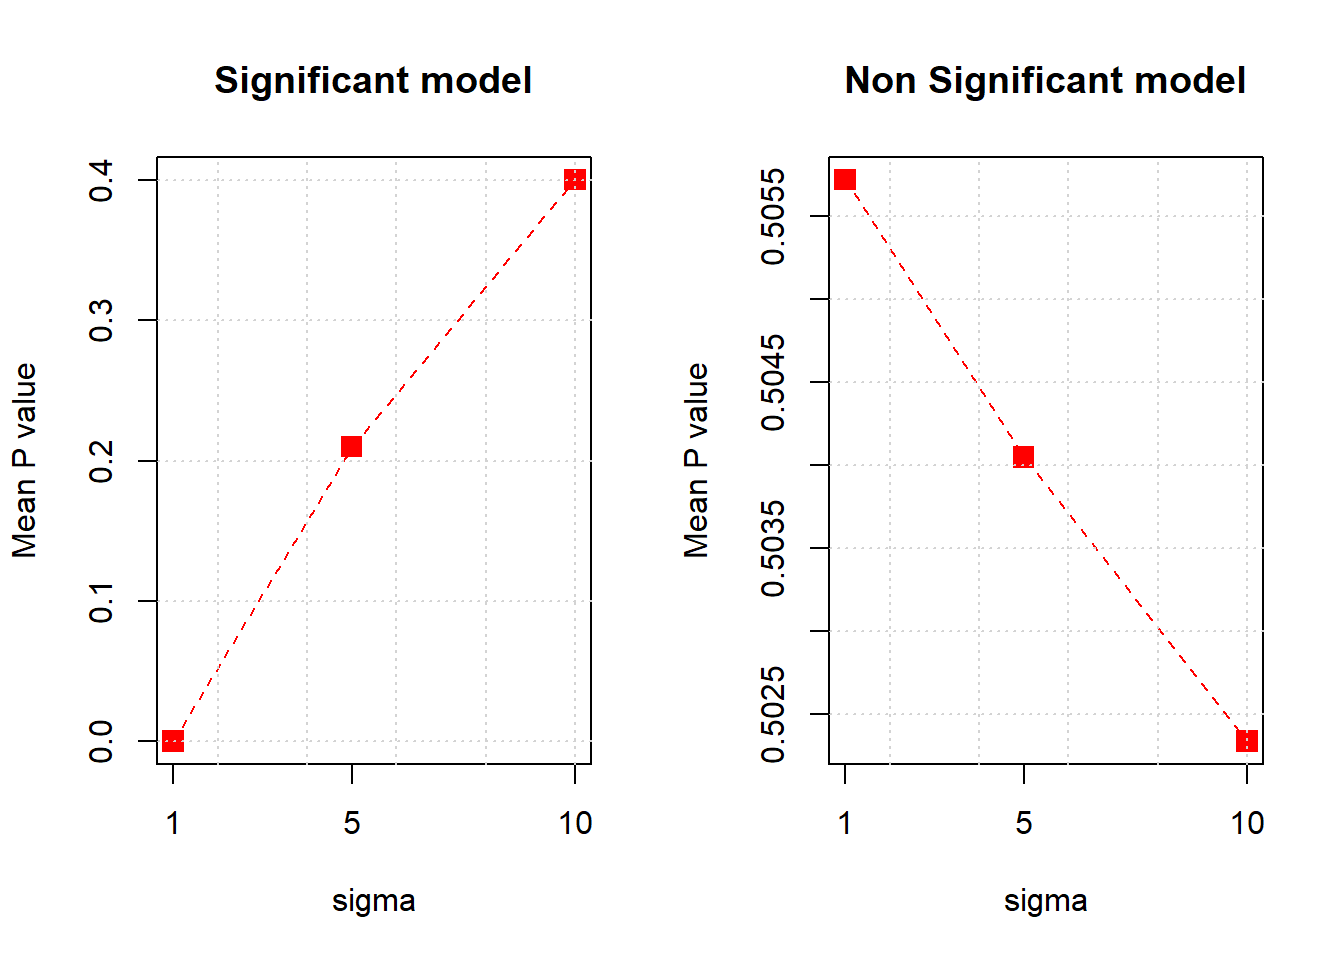
\includegraphics[width=35.06in,height=3.62in,keepaspectratio]{summer_proj_proposal_files/figure-latex/unnamed-chunk-4-1.png}

\begin{Shaded}
\begin{Highlighting}[]
\CommentTok{#Find rows with 0 values and set to NA}
\NormalTok{tmdb_movies_small[tmdb_movies_small}\OperatorTok{$}\NormalTok{budget }\OperatorTok{==}\StringTok{ }\DecValTok{0}\NormalTok{, }\StringTok{"budget"}\NormalTok{ ] =}\StringTok{ }\OtherTok{NA}
\NormalTok{tmdb_movies_small[tmdb_movies_small}\OperatorTok{$}\NormalTok{revenue }\OperatorTok{==}\StringTok{ }\DecValTok{0}\NormalTok{, }\StringTok{"revenue"}\NormalTok{ ] =}\StringTok{ }\OtherTok{NA}
\NormalTok{tmdb_movies_small[tmdb_movies_small}\OperatorTok{$}\NormalTok{popularity }\OperatorTok{==}\StringTok{ }\DecValTok{0}\NormalTok{, }\StringTok{"popularity"}\NormalTok{ ] =}\StringTok{ }\OtherTok{NA}
\CommentTok{#tmdb_movies_small[tmdb_movies_small$vote_count == 0, "vote_average" ] = NA}
\NormalTok{tmdb_movies_small}\OperatorTok{$}\NormalTok{original_language =}\StringTok{ }\KeywordTok{as.factor}\NormalTok{(tmdb_movies_small}\OperatorTok{$}\NormalTok{original_language)}

\CommentTok{#remove invalid rows}
\NormalTok{tmdb_movies_small =}\StringTok{  }\KeywordTok{na.omit}\NormalTok{(tmdb_movies_small)}
\end{Highlighting}
\end{Shaded}

\begin{Shaded}
\begin{Highlighting}[]
\CommentTok{#Fit a simple  model and print summary}
\NormalTok{boxoffice_model_}\DecValTok{1}\NormalTok{ =}\StringTok{ }\KeywordTok{lm}\NormalTok{(revenue }\OperatorTok{~}\StringTok{  }\NormalTok{budget}\OperatorTok{+}\NormalTok{popularity , tmdb_movies_small)}
\KeywordTok{summary}\NormalTok{(boxoffice_model_}\DecValTok{1}\NormalTok{)}
\end{Highlighting}
\end{Shaded}

\begin{verbatim}
## 
## Call:
## lm(formula = revenue ~ budget + popularity, data = tmdb_movies_small)
## 
## Residuals:
##       Min        1Q    Median        3Q       Max 
## -1.04e+09 -4.66e+07 -7.09e+06  2.35e+07  1.99e+09 
## 
## Coefficients:
##              Estimate Std. Error t value Pr(>|t|)    
## (Intercept) -2.68e+07   2.94e+06   -9.13   <2e-16 ***
## budget       2.30e+00   5.14e-02   44.69   <2e-16 ***
## popularity   1.88e+06   6.31e+04   29.87   <2e-16 ***
## ---
## Signif. codes:  0 '***' 0.001 '**' 0.01 '*' 0.05 '.' 0.1 ' ' 1
## 
## Residual standard error: 117000000 on 3226 degrees of freedom
## Multiple R-squared:  0.606,  Adjusted R-squared:  0.606 
## F-statistic: 2.49e+03 on 2 and 3226 DF,  p-value: <2e-16
\end{verbatim}

A simple additive model above was used to predict revenue based on
popularity and budget of the movie. The predictors seems to be
significant, our objective is to improve this simplistic model in final
report of this project.

\end{document}
